\section{Formální jazyky}\label{sec:jazyky}

Nyní, když jsme si vysvětlili základy konečných automatů a~jejich roli ve zpracovávání formálních jazyků, můžeme se hlouběji ponořit do problematiky formálních jazyků samotných. Tyto jazyky jsou totiž základem pro popis množin řetězců a~jsou klíčové pro definování toho, co automaty rozpoznávají.

Formální jazyky lze chápat jako abstraktní systémy pro popis pravidel, podle kterých jsou vytvářeny řetězce symbolů. Jsou zásadní nejen pro teorii automatů, ale také pro návrh programovacích jazyků a~kompilátorů. V~následujících částech se zaměříme na různé typy gramatik, které jsou základem pro definici formálních jazyků, a~ukážeme si, jak konečné automaty mohou tyto jazyky rozpoznávat a~zpracovávat.

Pro začátek si (jako vždy) uvedeme definice některých základních pojmů.
\begin{definition}
    Máme neprázdnou množinu znaků $\Sigma$, tzv. \textbf{abecedu}.
    \begin{itemize}
        \item \textbf{Slovo (řetězec)} je libovolná konečná posloupnost znaků ze $\Sigma$.
        \item \textbf{Prázdné slovo} je slovo neobsahující žádné znaky\footnote{Symbol $\lambda$ zde představuje speciální znak zastupující prázdné slovo. Neuvažujeme jej tedy jako součást abecedy $\Sigma$, tzn. $\lambda\notin\Sigma$.}, značíme $\lambda$.
        \item \textbf{Množina všech slov v abecedě $\Sigma$} se značí $\Sigma^*$.
        \item \textbf{Jazyk} je libovolná podmnožina slov $L\subseteq\Sigma$. Říkáme, že jazyk $L$ je \emph{nad abecedou $\Sigma$} (viz obrázek \ref{fig:jazyk}).
        \begin{figure}[h]
            \centering
            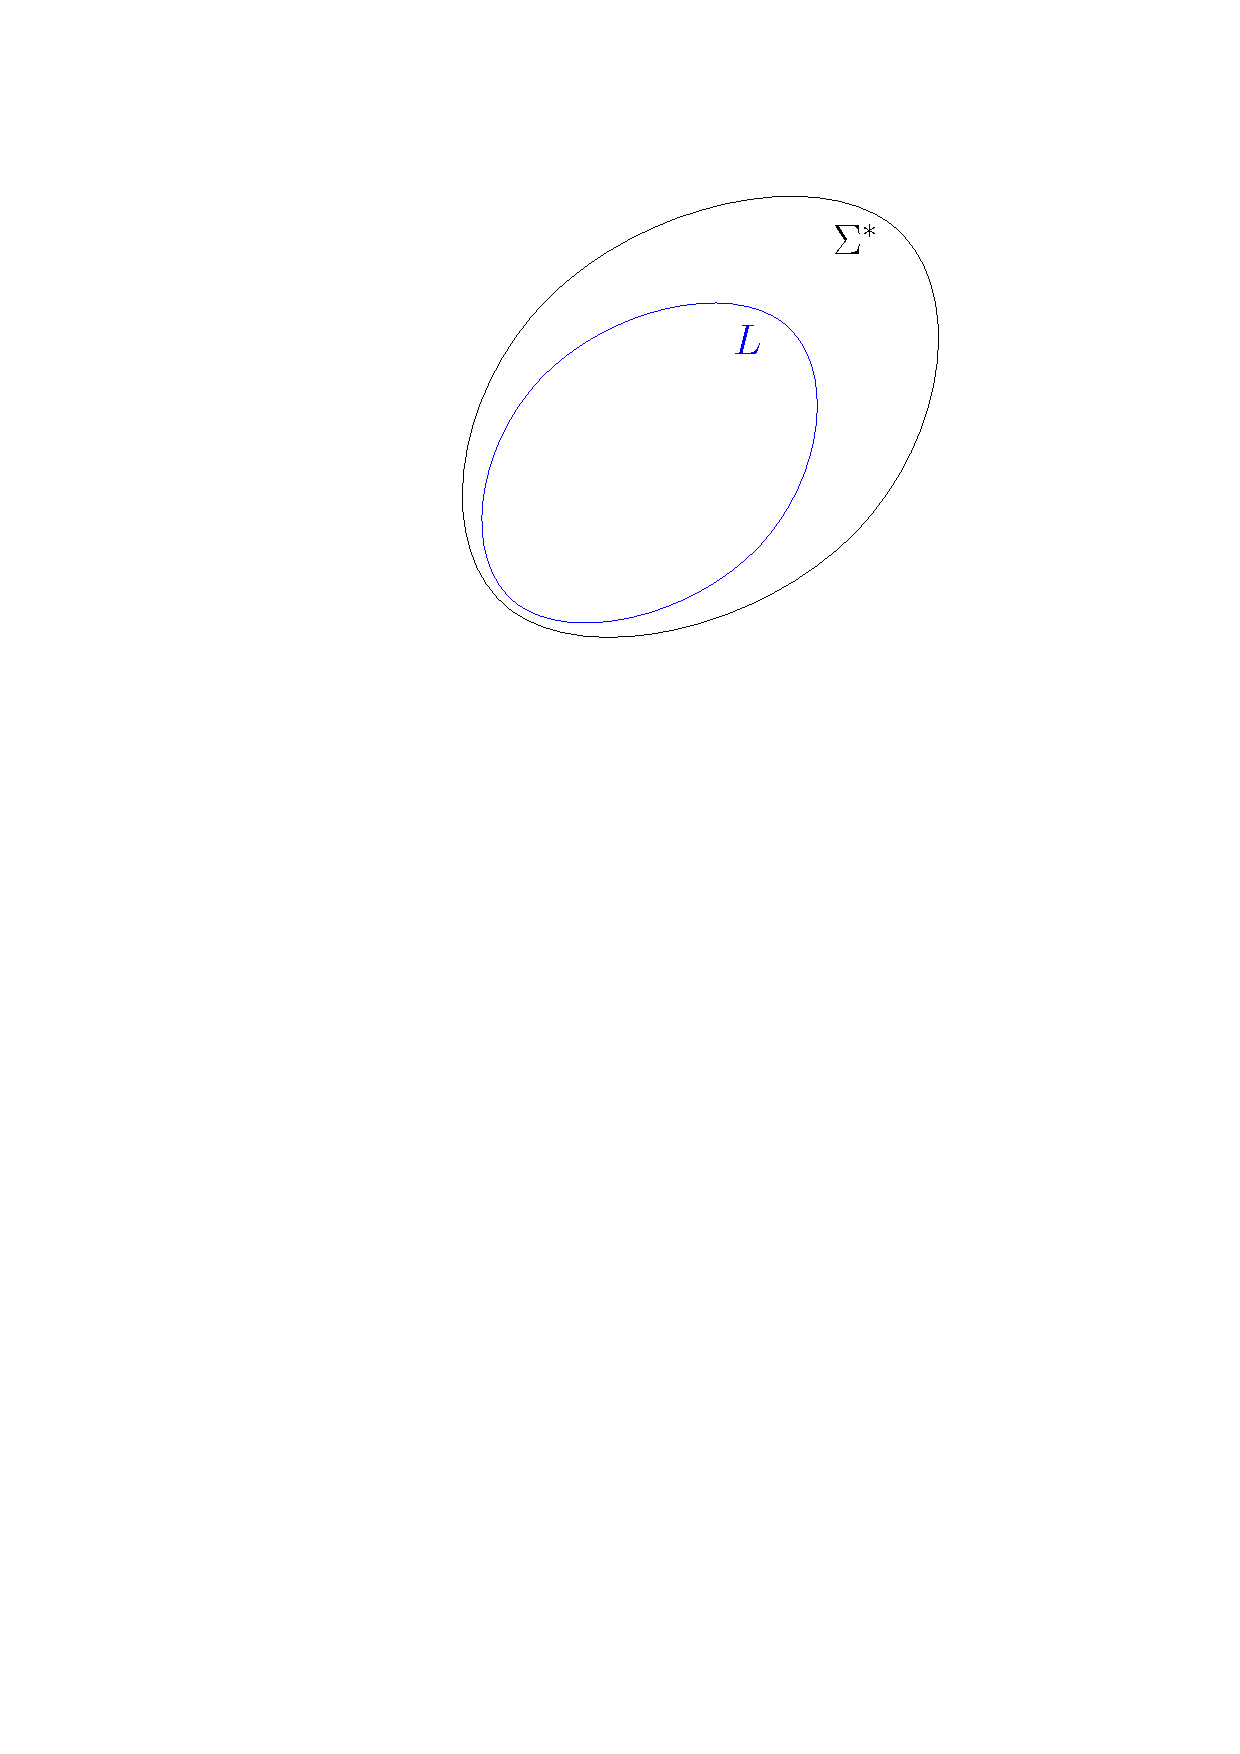
\includegraphics[scale=.7]{03-automaty/images/ch03_jazyk.pdf}
            \caption{Obecný jazyk $L$ nad abecedou $\Sigma$.}
            \label{fig:jazyk}
        \end{figure}
        \item \textbf{Délka slova} $w$ (tzn. počet znaků) se značí $|w|$.
        \item \textbf{Konkantenace} slov $u,v\in\Sigma^*$, kde $u=u_1u_2\dots u_n$ a $v=v_1v_2\dots v_m$ je slovo
        \[uv=u_1u_2\dots u_nv_1v_2\dots v_m.\]
        \item \textbf{$n$-tá mocnina} slova $u\in\Sigma^*$ je slovo
        \[u^n=\underbrace{uu\dots u}_{\text{$n$-krát}},\]
        kde $n\in\N_0$. Speciálně $u^0=\lambda$.
    \end{itemize}
\end{definition}
Podívejme se na jednoduchý příklad.
\begin{example}
    Mějme dvouznakovou abecedu $\Sigma=\set{a,b}$.
    \begin{itemize}
        \item Např. slovem v takto zadané abecedě $\Sigma$ je $w=abba$. Tzn. $|w|=4$.
        \item Množina všech slov\footnote{Je pochopiltené, že tato množina je nekonečná (délka slov není nijak omezená).} $\Sigma^*=\set{\lambda,a,b,aa,ab,ba,bb,aaa,aab,aba,\dots}$.
        \item Jednoduchý příklad jazyka nad abecedou $\Sigma$ je $L_1=\Sigma^*$, tedy všechna možná slova sestávající ze znaků $a,b$.
        \item Dalším příkladem může být např. jazyk $L_2=\set{w\in\Sigma^*\mid |w|\leqslant 2}$. Jazyk $L_2$ tedy obsahuje všechna slova délky nejvýše $2$, tj.
        \[L_2=\set{\lambda,a,b,aa,ab,ba,bb}.\]
        \item Pátá mocnina slova $w=abba$:
        \[w^5=abbaabbaabbaabbaabba.\]
        \item Konkantenace slov $u=aabb$ a $v=bbaa$
        \[uv=aabbbbaa.\]
    \end{itemize}
\end{example}

Jazyky nejsou v matematickém pojetí nic jiné než množiny objektů, tedy v tomto případě slov.
\begin{example}
    Další příklady jazyků:
    \begin{itemize}
        \item Jazyk $U=\set{w\in\Sigma^*\mid w\subseteq\set{X,Y}^*}$ obsahující všechna \emph{slova sestávající pouze z velkých písmen} nad abecedou $\Sigma=\set{x,y,X,Y}$.
        \item Jazyk $N=\set{u\in\Lambda^*\mid |u|\geqslant 1}$ obsahující všechna \emph{neprázdná slova} nad obecnou abecedou $\Lambda$ (může být jakákoliv).
        \item Jazyk $Z=\set{0^n1^n\mid n\in\N}$ nad abecedou $\Omega=\set{0,1}$.
    \end{itemize}
\end{example}